%%%% Better Poster latex template example v1.0 (2019/04/04)
%%%% GNU General Public License v3.0
%%%% Rafael Bailo
%%%% https://github.com/rafaelbailo/betterposter-latex-template
%%%% 
%%%% Original design from Mike Morrison
%%%% https://twitter.com/mikemorrison

\documentclass[a1paper,fleqn]{betterposter}
%%%% Uncomment the following commands to customise the format

%% Setting the width of columns
% Left column
%\setlength{\leftbarwidth}{0.25\paperwidth}
% Right column
%\setlength{\rightbarwidth}{0.25\paperwidth}

%% Setting the column margins
% Horizontal margin
%\setlength{\columnmarginvertical}{0.05\paperheight}
% Vertical margin
%\setlength{\columnmarginhorizontal}{0.05\paperheight}
% Horizontal margin for the main column
%\setlength{\maincolumnmarginvertical}{0.15\paperheight}
% Vertical margin for the main column
\setlength{\maincolumnmarginhorizontal}{0.04\paperheight}

%% Changing font sizes
% Text font
%\renewcommand{\fontsizestandard}{\fontsize{28}{35} \selectfont}
% Main column font
\renewcommand{\fontsizemain}{\fontsize{80.00}{120.00} \selectfont}
% Title font
%\renewcommand{\fontsizetitle}{\fontsize{28}{35} \selectfont}
% Author font
%\renewcommand{\fontsizeauthor}{\fontsize{28}{35} \selectfont}
% Section font
%\renewcommand{\fontsizesection}{\fontsize{28}{35} \selectfont}

%% Changing font sizes for a specific text segment
% Place the text inside brackets:
% {\fontsize{28}{35} \selectfont Your text goes here}

%% Changing colours
% Background of side columns
%\renewcommand{\columnbackgroundcolor}{black}
% Font of side columns
%\renewcommand{\columnfontcolor}{gray}
% Background of main column
\renewcommand{\maincolumnbackgroundcolor}{empirical}
%\renewcommand{\maincolumnbackgroundcolor}{theory}
%\renewcommand{\maincolumnbackgroundcolor}{methods}
%\renewcommand{\maincolumnbackgroundcolor}{intervention}
% Font of main column
%\renewcommand{\maincolumnfontcolor}{gray}

\begin{document}
\betterposter{
%%%%%%%% MAIN COLUMN

\maincolumn{
%%%% Main space

\begin{flushleft}
Does
\textbf{purely functional programming} offer benefits 
for the
\textbf{design} and \textbf{implementation} of
\textbf{distributed stream-processing} systems?
\end{flushleft}

}{
%%%% Bottom space

%% QR code
\qrcode{img/qrcode}{img/smartphoneWhite}{
\textbf{Take a picture} to read more
\\at the STrIoT.org website
}
% Smartphone icon
% Author: Freepik
% Retrieved from: https://www.flaticon.com/free-icon/smartphone_65680

%% Compact QR code (comment the previous command and uncomment this one to switch)
%\compactqrcode{img/qrcode}{
%\textbf{Take a picture} to
%\\download the full paper
%}

}

}{
%%%%%%%% LEFT COLUMN

\title{StrIoT}
\author{Jonathan Dowland}
\institution{Newcastle University}

{\color{gray}\textit{Supervisor: Paul Watson}}

Many modern applications require timely processing of data arriving at high
speed (e.g. IoT domains) and may also need to meet requirements of:
reliability; security; energy efficiency (e.g. prolong sensor battery life) or
privacy.

In combination these make the design and management of solutions very challenging.

We are exploring whether declarative, purely-functional programming can
produce more efficient deployments than traditional approaches. 

\section{StrIoT Architecture}
\textit{Paul Watson, Andrey Mokhov}
\begin{center}
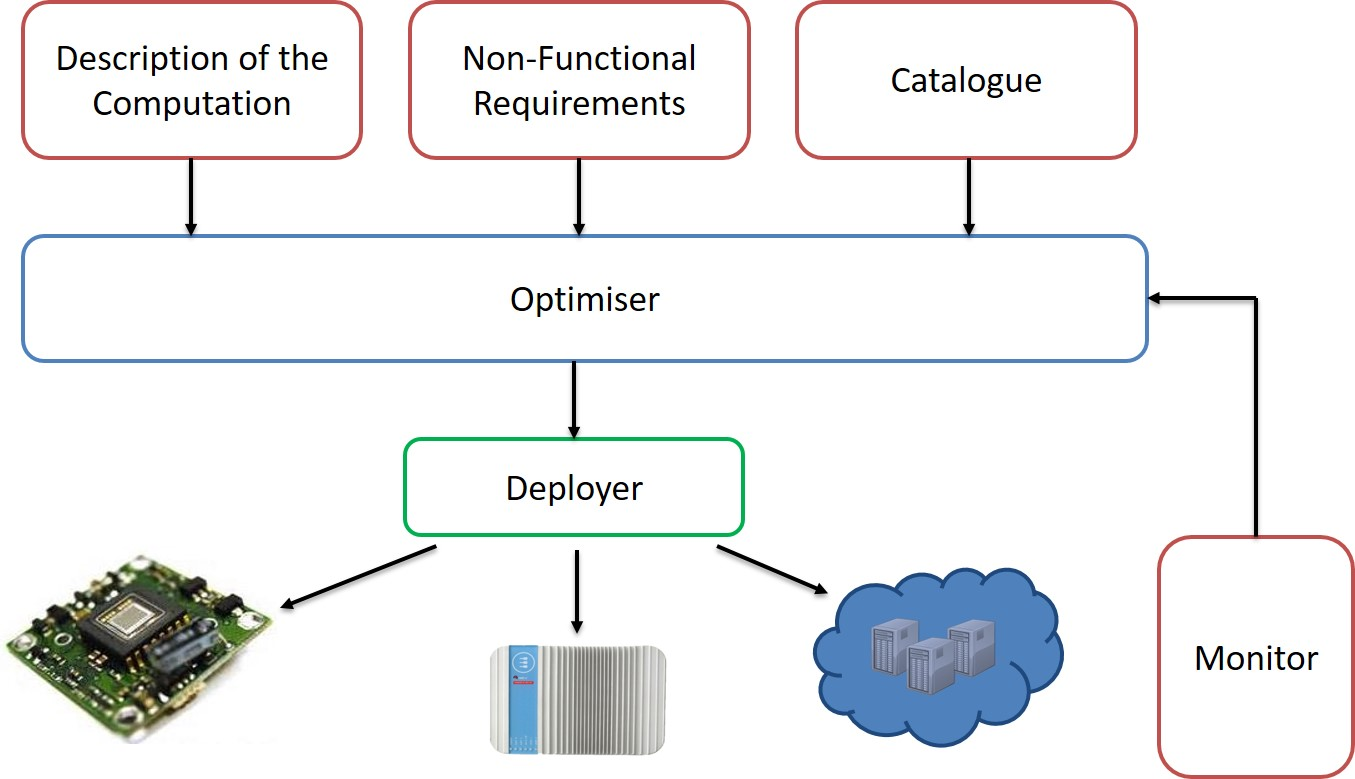
\includegraphics[width=\textwidth]{img/draft_paper_diagram}
\end{center}

\section{Logical Optimisation}

I'm focussing on logical optimisation:
rewriting a stream-processing program to
better meet non-functional requirements whilst preserving its functional
definition.

%% This fills the space between the content and the logo
\vfill

%% Institution logo

\includegraphics[width=\textwidth]{img/logo}\\

}{
%%%%%%%% RIGHT COLUMN

\section{Work completed}

\begin{itemize}
    \item Designed and built prototype stream-processing system
        that accepts a stream-processing definition, partitions
        it into separate programs for deployment via Docker

    \item Derived 24 stream rewrite rules
        for use in logical optimisation

\end{itemize}

\section{Example rewrite}

Input stream-graph:

\begin{center}
% this is coming out at approx a4 size so should be legible
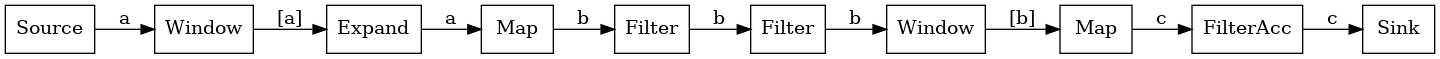
\includegraphics[width=\textwidth]{img/before}
\end{center}

Apply rewrites:

\[
\begin{aligned}
filter\ a\ \cdot\ filter\ b\ =
\\    filter\ (\lambda\ x \rightarrow\ a\ x\ \&\&\ b\ x)
\end{aligned}
\]

\[
    filter\ p\ \cdot\ map\ f\ =\ map\ f\ \cdot\ filter\ (p\ \cdot\ f)
\] 

Result:

\begin{center}
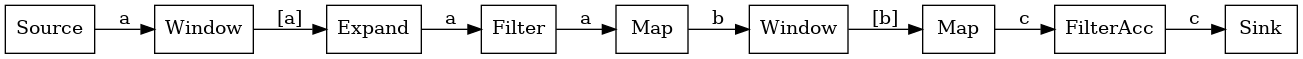
\includegraphics[width=\textwidth]{img/after}
\end{center}

\section{Next Steps}

\begin{itemize}
    \item Evaluation of stream representations
    \item Build Logical Optimiser (including a cost model for evaluating )
    \item Automatic stream partitioning
\end{itemize}

\vfill
\author{jon.dowland@ncl.ac.uk}

}
\end{document}
